\section{Modern Applications of Boolean Algebra}
Beyond its fundamental role in hardware minimization, Boolean algebra remains an essential tool in cryptography, biological systems, and data management. Binary logic facilitates efficient decision-making, secure computation, and high-performance structured search within modern computational frameworks \cite{picek2016cryptographic}.

\subsection{Cryptography}
Boolean functions $f: \{0,1\}^n \to \{0,1\}$ serve as the primary building blocks for symmetric cryptographic systems. They are specifically utilized in the design of Substitution-boxes (S-boxes) for block ciphers like the Advanced Encryption Standard (AES) and as filter generators in stream ciphers. To ensure resistance against cryptanalysis, researchers optimize these functions for specific properties:
\begin{itemize}
    \item \textbf{Nonlinearity:} High nonlinearity is required to prevent linear cryptanalysis, ensuring the output cannot be approximated by a linear combination of input bits.
    \item \textbf{Algebraic Degree:} A high algebraic degree is necessary to defend against higher-order differential attacks.
    \item \textbf{Correlation Immunity:} This property ensures the output is statistically independent of subsets of input bits, protecting against correlation attacks \cite{tu2012boolean}.
\end{itemize}

\subsection{Biological Network Modeling}
In bioinformatics and systems biology, Boolean algebra is used to model Gene Regulatory Networks (GRNs) by treating molecular components as discrete binary variables. A gene is represented as $1$ (active/expressed) or $0$ (inactive/repressed). The regulatory interactions such as activation or inhibition are defined by Boolean functions that determine the state of a node based on the current state of its regulators \cite{puvsnik2022review}.

\begin{figure}[h]
    \centering
    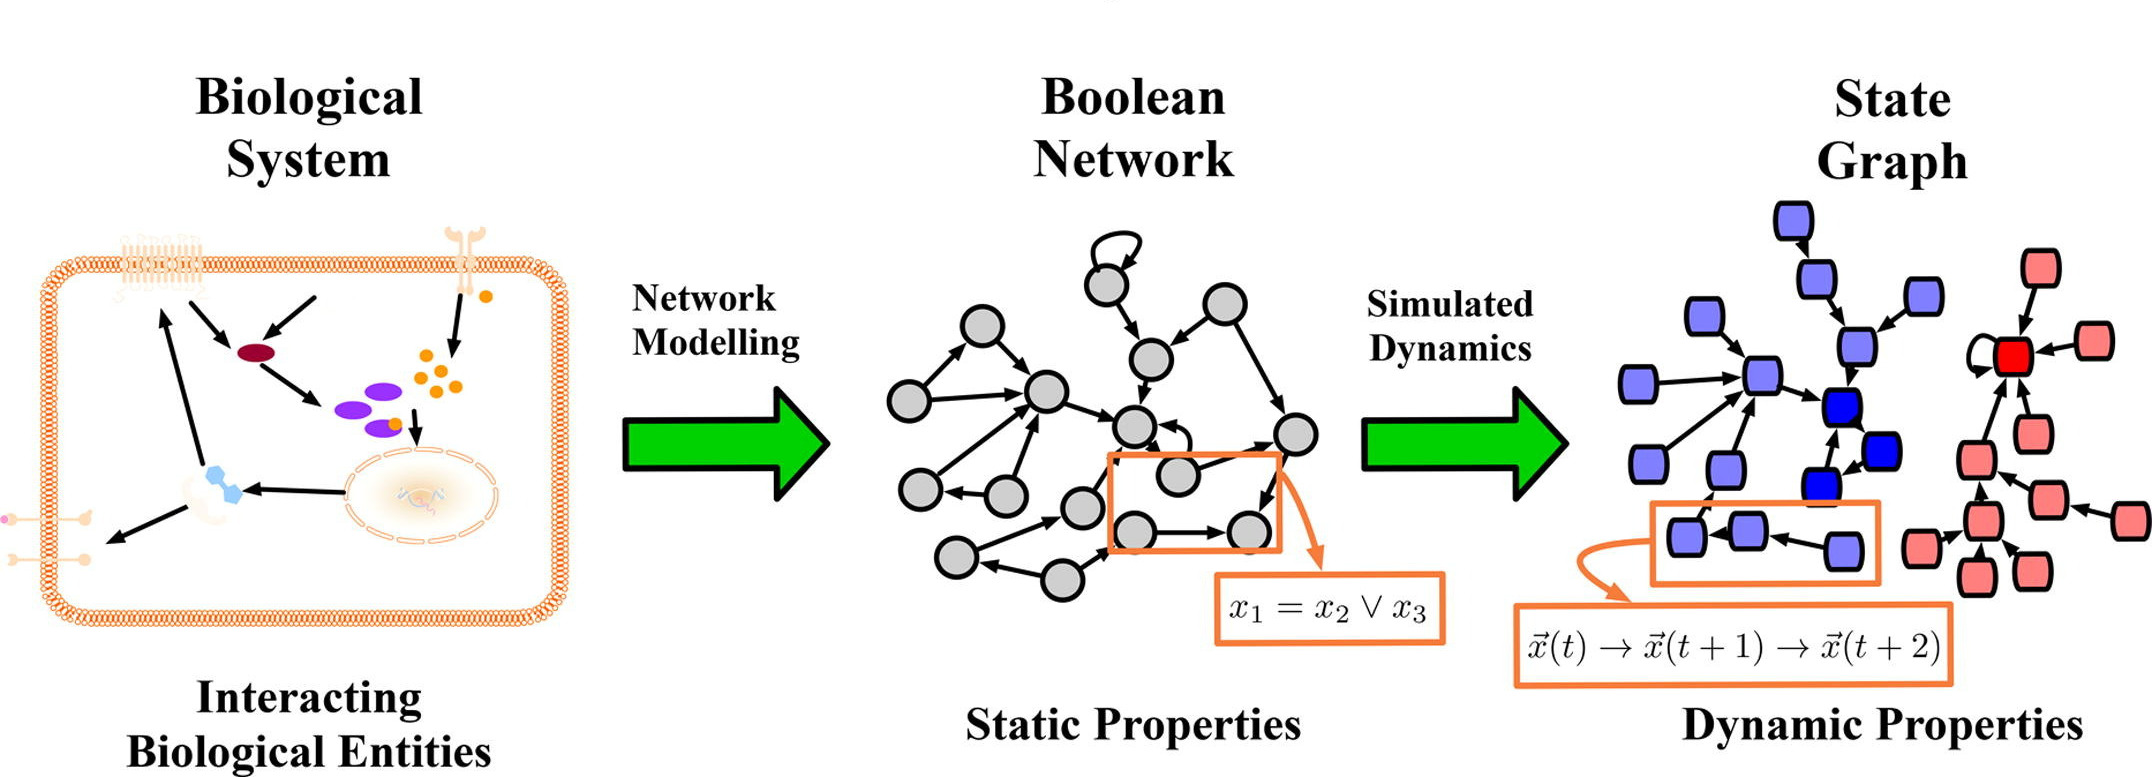
\includegraphics[width=0.8\textwidth]{images/biological-boolean-network-modelling.jpg}
    \caption{State transition graph and Boolean logic in a gene regulatory network modeling cell state stability.}
    \label{fig:bio_boolean}
\end{figure}

\bigskip
\textbf{Example: Regulatory Logic and Attractors}
A core strength of this model, as noted by Schwab et al. \cite{schwab2020concepts}, is the ability to map the \textit{state space} of a cell. For instance, if Gene A activates Gene B, but Gene B inhibits Gene A, the system can be modeled as:
\begin{itemize}
    \item $A_{t+1} = \text{NOT } B_t$
    \item $B_{t+1} = A_t$
\end{itemize}

As visualized in Figure \ref{fig:bio_boolean}, by iterating these logical transitions, researchers identify \textbf{Attractors}—stable cycles or steady states that correspond to biological phenotypes, such as a cell reaching maturity or responding to environmental stress. This allows for the simulation of complex "what-if" scenarios, such as predicting the effects of a gene knockout (permanently setting a variable to 0) on the entire network topology \cite{schwab2020concepts}.

\subsection{Information Retrieval and Search}
Modern search engines and digital libraries rely on Boolean logic for query formulation. By combining keywords with AND, OR, and NOT operators, systems can precisely include or exclude documents. Research indicates that logical query transformations and refinements significantly improve both recall (finding all relevant documents) and precision (minimizing irrelevant results) in systematic evidence-based research \cite{alharbi2020refining}.

\subsection{Database and Data Filtering}
Boolean logic is central to database management systems (DBMS), where it is used in selection rules and indexing strategies to process large datasets efficiently.

\bigskip
\textbf{Example: Multi-Criteria SQL Filtering}
Consider a library database where a user seeks specific research papers. A Boolean expression for this search might be:
\begin{center}
    \textit{(Category = 'Physics' \textbf{OR} Category = 'Engineering') \textbf{AND} \textbf{NOT} (Status = 'Loaned')}
\end{center}

In this application, the system evaluates each record:
\begin{enumerate}
    \item \textbf{Disjunction (OR):} Identifies all items in either the Physics or Engineering departments.
    \item \textbf{Negation (NOT):} Identifies all items currently available on the shelf.
    \item \textbf{Conjunction (AND):} Intersects these two sets to return only the available items in the specified fields.
\end{enumerate}
This logical structure allows database engines to use bitmasking to filter millions of rows in milliseconds, demonstrating that Boolean algebra is as critical to modern software efficiency as it is to hardware design \cite{gfg2026boolean}.